% ==============================================
% CFD Tutorial Template: OpenFOAM Terminal Basics
% Class: scrartcl (KOMA-Script) - optimized for tutorials
% Content: pitzDaily with simpleFoam
% ==============================================

\documentclass[
    parskip=half,      % Space between paragraphs (better for steps)
    DIV=12,            % Optimal margins for readability
    headings=normal,   % Professional heading sizes
    fontsize=11pt,     % Slightly larger for screen reading
    english            % Language setting
]{scrartcl}

% ========== ESSENTIAL PACKAGES ==========
\usepackage[utf8]{inputenc}
\usepackage[T1]{fontenc}
\usepackage{lmodern}
\usepackage{geometry}
\usepackage{tikz}
\usepackage{microtype}           % Superior typography
\usepackage{graphicx}            % For screenshots (optional)
\usepackage{xcolor}              % Color coding
\usepackage{listings}            % Code listings
\usepackage{siunitx}             % Proper units: \si{\meter\per\second}
\usepackage{amsmath}             % Math equations
\usepackage{hyperref}            % Clickable links
\usepackage{url}
\usepackage{booktabs}            % Professional tables
\usepackage{caption}             % Better figure captions
\usepackage[english]{babel}
\usepackage{float}

% ========== CUSTOM COLORS ==========
\definecolor{codebg}{RGB}{240, 245, 250}
\definecolor{cmdcolor}{RGB}{0, 100, 0}
\definecolor{outputcolor}{RGB}{100, 100, 150}
\definecolor{warningcolor}{RGB}{180, 0, 0}
\definecolor{tipcolor}{RGB}{0, 100, 50}

% ========== CODE LISTING SETUP ==========
\lstset{
	backgroundcolor=\color{codebg},
	basicstyle=\ttfamily\small,
	breaklines=true,
	frame=single,
	captionpos=b,
	rulecolor=\color{gray!30},
	tabsize=2,
	showstringspaces=false
}

% Custom style for terminal commands
\lstdefinestyle{terminal}{
	basicstyle=\ttfamily\small\color{cmdcolor},
	backgroundcolor=\color{black!5},
	frame=none,
	columns=fullflexible
}

% Custom style for OpenFOAM files
\lstdefinestyle{openfoam}{
	language=C++,
	morekeywords={dimensions, internalField, boundaryField, type, value},
	keywordstyle=\color{blue},
	commentstyle=\color{gray!50}\itshape
}

\lstdefinestyle{output}{
	backgroundcolor=\color{black!5},
	basicstyle=\ttfamily\small\color{outputcolor},
	frame=none,
	breaklines=true
}
% ========== HYPERREF SETUP ==========
\hypersetup{
	colorlinks=true,
	linkcolor=blue,
	citecolor=green,
	filecolor=magenta,
	urlcolor=cyan,
	pdftitle={OpenFOAM Tutorial: pitzDaily with simpleFoam},
	pdfauthor={Your Name},
	pdfsubject={CFD with OpenFOAM},
	pdfkeywords={OpenFOAM, CFD, simpleFoam, pitzDaily, terminal}
}


\newcommand{\warning}[1]{\par\vspace{5pt}\noindent\textcolor{red}{\textbf{WARNING:}} #1\par\vspace{3pt}}
\newcommand{\tip}[1]{\par\vspace{5pt}\noindent\textcolor{green!50!black}{\textbf{TIP:}} #1\par\vspace{3pt}}
\newcommand{\important}[1]{\par\vspace{5pt}\noindent\textcolor{blue}{\textbf{IMPORTANT:}} #1\par\vspace{3pt}}                    

% ========== CUSTOM COMMANDS ==========
\newcommand{\terminalcmd}[1]{\textbf{\texttt{\textcolor{cmdcolor}{#1}}}}
\newcommand{\ofkeyword}[1]{\textbf{\textcolor{blue}{#1}}}
\newcommand{\filename}[1]{\texttt{\textcolor{purple}{#1}}}
\newcommand{\commandexample}[1]{\vspace{5pt}\hspace{10pt}\terminalicon\ \terminalcmd{#1}\vspace{5pt}}
\newcommand{\key}[1]{\texttt{\textbf{#1}}}


% ========== DOCUMENT START ==========
\begin{document}

% ========== TITLE PAGE ==========
\title{Tutorial \#1: OpenFOAM with terminal}
\subtitle{Incompressible Steady Flow: pitzDaily with simpleFoam}
\subject{Open Source CFD }
\author{Robert Castilla \\ Department of Fluid Mechanics}
\date{2025-26 \\ Version 1.0}
\publishers{Learning Objectives:
\begin{itemize}
    \item Navigate OpenFOAM case directory structure
    \item Understand basic OpenFOAM file formats
    \item Run a simple steady-state simulation
    \item Analyze basic results in terminal
    \item Troubleshoot common errors
\end{itemize}}

\maketitle

% ========== ABSTRACT ==========
\begin{abstract}
This tutorial introduces the fundamental workflow of Computational Fluid Dynamics (CFD) using OpenFOAM in a terminal environment. Through the classic \filename{pitzDaily} case with the \terminalcmd{simpleFoam} solver, students will learn to set up, run, and analyze an incompressible steady-state flow simulation. No graphical interface is required—all operations are performed via command line, making this ideal for remote servers and building core CFD skills.
\end{abstract}

\tableofcontents
\newpage

% ========== SECTION 1: INTRODUCTION ==========
\section{Introduction and Theoretical Background}

\subsection{What is pitzDaily?}
The \filename{pitzDaily} case simulates 2D steady, turbulent flow in a backward-facing step configuration. It's included in the OpenFOAM tutorials and serves as an excellent starting point due to its:
\begin{itemize}
    \item Simple geometry but interesting physics (recirculation zone)
    \item Complete setup with all necessary files
    \item Quick runtime (minutes on most computers)
\end{itemize}

\begin{figure}[h]
	\begin{center}
		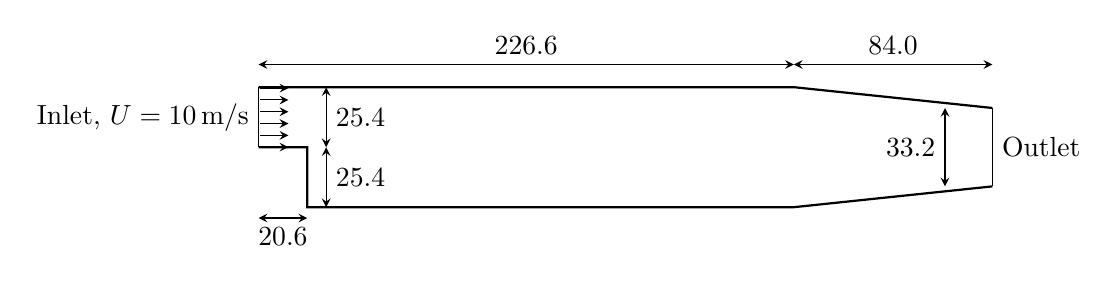
\begin{tikzpicture}[scale=0.03]
	% Draw the backward-facing step geometry
	\draw[thick] (-20.6,0) -- (0,0) -- (0,-25.4) -- (206,-25.4) -- (290,-16.6); % Lower
	\draw[thick] (-20.6,25.4) -- (0,25.4) -- (206,25.4) -- (290,16.6); % Upper
	\draw[thin] (-20.6,0) -- (-20.6,25.4) node[midway, left]{Inlet, $U = \qty{10}{m/s}$}; % Inlet
	\draw[thin] (290,-16.6) -- (290,16.6) node[midway, right]{Outlet}; % Outlet
	
	% Flow direction
	\foreach \y in {-0, 5, 10, 15, 20, 25} 
	\draw[-stealth] (-20,\y) -- ++(12,0);
	
	% Dimensions
	\draw[thin,stealth-stealth] (-20.6,35) -- (206,35) node[midway, above]{226.6}; 
	\draw[thin,stealth-stealth] (206,35) -- (290,35) node[midway, above]{84.0};
	\draw[thin,stealth-stealth] (270,-16.6) -- (270,16.6) node[midway, left]{33.2};
	\draw[thin,stealth-stealth] (8,0) -- (8,25.4) node[midway, right]{25.4};
	\draw[thin,stealth-stealth] (8,0) -- (8,-25.4) node[midway, right]{25.4};
	\draw[thin,stealth-stealth] (-20.6,-30) -- (0,-30) node[midway, below]{20.6};
\end{tikzpicture}
	\end{center}
	\caption{pitzDaily geometry. Lengths are in millimeter.}
\end{figure}

More information can be found on the \hyperlink{https://www.openfoam.com/documentation/tutorial-guide/3-compressible-flow/3.1-steady-turbulent-flow-over-a-backward-facing-step}{OpenFOAM website}.
\subsection{Governing Equations}
The \terminalcmd{simpleFoam} solver implements the incompressible Reynolds-Averaged Navier-Stokes (RANS) equations:

\begin{equation}
\nabla \cdot \mathbf{U} = 0
\end{equation}

\begin{equation}
\nabla \cdot (\mathbf{U} \mathbf{U})  = -\nabla \left(\frac{p}{\rho}\right) + \nabla \cdot (\nu_{\text{eff}} \nabla \mathbf{U})
\end{equation}

where $\nu_{\text{eff}} = \nu + \nu_t$ is the effective viscosity (molecular + turbulence viscosity).

Note that, since the fluid is incompressible,  instead of pressure $p$, this equation
deals with kinematic pressure , $\frac{p}{\rho}$, that has units of \unit{m^2/s^2}. 

\important{The solver \terminalcmd{simpleFoam} keeps the name $p$ for the kinematic pressure.}

\newpage

\subsection{Case Overview}
\begin{table}[h]
\centering
\begin{tabular}{@{}ll@{}}
\toprule
\textbf{Parameter} & \textbf{Value} \\
\midrule
Solver & \terminalcmd{simpleFoam} (steady, incompressible) \\
Turbulence model & $k$-$\epsilon$ (standard) \\
Flow regime & Turbulent \\
Geometry & 2D backward-facing step \\
Reynolds number & $\sim 2 \times 10^4$ (based on step height) \\
Expected runtime & 5-10 seconds \\
\bottomrule
\end{tabular}
\caption{pitzDaily case specifications}
\label{tab:case_specs}
\end{table}

% ========== SECTION 2: TERMINAL SETUP ==========
\section{Terminal Environment Setup}

\subsection{Accessing OpenFOAM}
Open your terminal and verify OpenFOAM is available:

\begin{lstlisting}[style=terminal]
foamVersion
\end{lstlisting}

\important{If you see "command not found," you may need to source the OpenFOAM environment first:}
\begin{lstlisting}[style=terminal]
# For system-wide installation
source /usr/lib/openfoam/openfoam-2312/etc/bashrc
\end{lstlisting}

\subsection{Navigating to Tutorials}
OpenFOAM includes a comprehensive set of tutorials. Navigate to the incompressible tutorials:

\begin{lstlisting}[style=terminal]
# Go to OpenFOAM tutorials directory
cd $FOAM_TUTORIALS

# List available tutorials
ls

# Navigate to incompressible simpleFoam tutorials
cd incompressible/simpleFoam
\end{lstlisting}

% ========== SECTION 3: CASE EXPLORATION ==========
\section{Case Structure Exploration}

\subsection{Understanding OpenFOAM Directory Structure}

Copy the pitzDaily case in a local folder

\begin{lstlisting}[style=terminal]
	# Make a local folder
	mkdir -p $HOME/Tutorials/Tutorial_1
	
	# Copy the pitzDaily tutorial in this folder
	cp -r ./pitzDaily $HOME/Tutorials/Tutorial_1
	
	# Go to the tutorial place
	cd $HOME/Tutorials/Tutorial_1
\end{lstlisting}

\important{Never play with a tutorial in the OpenFOAM distribution home folder. Always make a copy. In this way you will have always a "clean" copy.}

Examine the pitzDaily case structure:

\begin{lstlisting}[style=terminal]
# Go to the pitzDaily case
cd pitzDaily

# List all contents with details
ls -la

# See the directory structure
tree -L 2
\end{lstlisting}

\important{Every OpenFOAM case has this standard structure:}
\begin{lstlisting}[style=openfoam]
	pitzDaily/
	|-- 0/           # Initial and boundary conditions
	|-- constant/    # Physical properties and mesh
	|   |-- polyMesh/   # Mesh files
	|   `-- transportProperties
	\-- system/      # Solution control
	    |-- controlDict
	    |-- fvSchemes
	    `-- fvSolution
\end{lstlisting}

\subsection{Examining Key Files}
Let's look at the most important configuration files:

\begin{enumerate}
	\renewcommand{\labelenumi}{\textbf{Step \arabic{enumi}:}}
\item \textbf{Initial Conditions (0/ directory)}:
\begin{lstlisting}[style=terminal]
# View velocity boundary conditions
cat 0/U

# View pressure boundary conditions  
cat 0/p

# View turbulence variables
cat 0/k
cat 0/epsilon
\end{lstlisting}

\item \textbf{Physical Properties}:
\begin{lstlisting}[style=terminal]
# Check fluid properties
cat constant/transportProperties
\end{lstlisting}

This shows:
\begin{lstlisting}[style=openfoam]
transportModel  Newtonian;

nu              1e-05;
\end{lstlisting}

\item \textbf{Solution Control}:
\begin{lstlisting}[style=terminal]
# Check solver settings
cat system/fvSolution

# Check discretization schemes
cat system/fvSchemes

# Check runtime control
cat system/controlDict
\end{lstlisting}
\end{enumerate}

\tip{Use \terminalcmd{less} or \terminalcmd{more} for longer files: \terminalcmd{less system/controlDict}}

% ========== SECTION 4: RUNNING THE SIMULATION ==========
\section{Running the Simulation}

\subsection{Pre-processing}
Before running, we need to generate the mesh:

\begin{lstlisting}[style=terminal]
# Generate the mesh using blockMesh, with the foamJob utility
foamJob -screen -log-app blockMesh

# Check mesh quality
foamJob -screen -log-app checkMesh
\end{lstlisting}

\warning{If \terminalcmd{blockMesh} fails, check for error messages. Common issues include missing dictionaries or syntax errors in \filename{system/blockMeshDict}.}

The utility \terminalcmd{foamJob} creates a log file.
 
\begin{lstlisting}[style=terminal]
	# Check the content of the log files
	less log.blockMesh
	less log.checkMesh
\end{lstlisting}

\subsection{Running simpleFoam}
Now run the simulation:

\begin{lstlisting}[style=terminal]
# Run the solver
foamJob -s -log-app simpleFoam

\end{lstlisting}

\subsection{Monitoring Convergence}
Monitor convergence:

\begin{lstlisting}[style=terminal]
# Watch residuals in real-time (if running in foreground)
# OR check the log file periodically:

# Show last 20 lines of residuals
tail -20 log.simpleFoam | grep "Solving for"

# Check final residuals
tail -50 log.simpleFoam | grep "Final residual"
\end{lstlisting}

Plot it using \terminalcmd{gnuplot}

\begin{lstlisting}[style=terminal]
	     # Generate residual files from the log file
	     foamLog log.simpleFoam
	
	     # Visualize the residuals of the main variables with gnuplot
	     gnuplot
gnuplot> set logscale y
gnuplot> plot  'logs/p_0'with lines ,'logs/Ux_0' with lines, 'logs/Uy_0' with lines, 'logs/epsilon_0' with lines, 'logs/k_0' with lines
\end{lstlisting}

You will get a picture similar to that in Figure \ref{fig:gnuplot}.

\begin{figure}[h]
	\centering
	\includegraphics[width=0.7\linewidth]{gnuplot}
	\caption{Plot of residuals}
	\label{fig:gnuplot}
\end{figure}

% ========== SECTION 5: POST-PROCESSING ==========
\section{Post-Processing in Terminal}

\subsection{Basic Results Examination}
OpenFOAM stores results in time directories. Examine the final results:

\begin{lstlisting}[style=terminal]
# List time directories
foamListTimes

# Go to final time directory (e.g., typically 281 for pitzDaily)
cd 281

# List available fields
ls

\end{lstlisting}

\subsection{Using OpenFOAM Command Line Tools}


Check field statistics:

\begin{lstlisting}[style=terminal]
# Go back to case root
cd ..

# Get pressure statistics
postProcess -func writeCellCentres
postProcess -func "patchAverage(name=inlet,p)"
postProcess -func minMaxMagnitudes
\end{lstlisting}

\important{Besides the screen, the information from \terminalcmd{postProcess} is also saved in the \filename{postProcessing} folder}

\tip{The command \terminalcmd{postProcess -list} will list all the functions available.}

\subsection{Basic Visualization in paraview}
Usually the program \terminalcmd{paraview} is used to visualize the results from OpenFOAM simulations. A wrapper \terminalcmd{paraFoam} is available to call the 
program after performing some internal operations


\begin{lstlisting}[style=terminal]
# Run the paraFoam script
paraFoam
\end{lstlisting}

\begin{figure}[h]
	\centering
	\includegraphics[width=\linewidth]{paraFoam001}
	\caption{Start screen for paraview, called with \terminalcmd{paraFoam}.}
	\label{fig:parafoam001}
\end{figure}

Click on the "Apply" button. By default, you will the pressure distribution (Figure \ref{fig:parafoam002}).

\begin{figure}[h]
	\centering
	\includegraphics[width=\linewidth]{paraFoam002}
	\caption{Pressure distribution of the flow.}
	\label{fig:parafoam002}
\end{figure}


% ========== SECTION 6: TROUBLESHOOTING ==========
\section{Common Issues and Troubleshooting}

\subsection{Error: "command not found"}
\begin{itemize}
\item \textbf{Cause}: OpenFOAM environment not sourced
\item \textbf{Solution}: 
\begin{lstlisting}[style=terminal]
source /path/to/OpenFOAM/etc/bashrc
\end{lstlisting}
\end{itemize}

\subsection{Error: "cannot find blockMeshDict"}
\begin{itemize}
\item \textbf{Cause}: Not in correct directory or file missing
\item \textbf{Solution}:
\begin{lstlisting}[style=terminal]
# Check current directory
pwd

# List contents of system
ls system
\end{lstlisting}
\end{itemize}

\subsection{Simulation Diverges (Residuals Grow)}
\begin{itemize}
\item \textbf{Cause}: Poor initial conditions or solver settings
\item \textbf{Solution}:
\begin{enumerate}
\item Reduce under-relaxation factors in \filename{system/fvSolution}
\item Check boundary conditions are physically realistic
\item Try running \terminalcmd{potentialFoam} first to get better initial fields
\end{enumerate}
\end{itemize}


% ========== SECTION 7: EXERCISES ==========
\section{Student Exercises and Extensions}

\subsection{Basic Exercises (Required)}
\begin{enumerate}

\item \textbf{Boundary Condition Modification}:
\begin{itemize}
\item Change inlet velocity from \SI{10}{\meter\per\second} to \SI{20}{\meter\per\second}
\item Update both \filename{0/U} and \filename{0/k}/\filename{0/epsilon} appropriately
\item \textbf{Question}: How does Reynolds number affect recirculation zone size?
\end{itemize}

\item \textbf{Turbulence Model Comparison}:
\begin{itemize}
\item Change from $k$-$\epsilon$ to $k$-$\omega$ SST in \filename{constant/turbulenceProperties}
\item \textbf{Question}: Which model converges faster? Which gives higher $k$ values?
\end{itemize}
\end{enumerate}

\subsection{Advanced Exercises (Optional)}
\begin{enumerate}
\item \textbf{Mesh Refinement Study}:
\begin{itemize}
\item Modify \filename{system/blockMeshDict} to double cells in x-direction
\item Compare velocity profiles at outlet
\end{itemize}

\item \textbf{Custom Geometry}:
\begin{itemize}
\item Create a simple 2D channel (modify blockMeshDict)
\item Reuse boundary conditions from pitzDaily
\item Compare pressure drop with analytical solution
\end{itemize}
\end{enumerate}

% ========== SECTION 8: DELIVERABLES ==========
\section{Deliverables and Assessment}

Submit the following to Moodle:

\subsection{Required Files}
\begin{enumerate}
\item Modified \filename{system/controlDict} with your student ID in comments
\item Final \filename{log.simpleFoam} file
\item Screen capture of terminal showing:
\begin{itemize}
\item Successful \terminalcmd{blockMesh} execution
\item Final residuals from \terminalcmd{simpleFoam}
\item Output of \terminalcmd{checkMesh}
\end{itemize}
\end{enumerate}

\subsection{Report Questions}
Answer the following in a PDF report:
\begin{enumerate}
\item What are the final residuals for $U_x$, $U_y$, $p$, $k$, and $\epsilon$?
\item How many iterations were needed for convergence?
\item What is the maximum pressure in the domain? Minimum?
\item Based on the recirculation zone length, what is the reattachment length?
\item If you changed parameters in exercises, discuss how they affected results.
\end{enumerate}

\subsection{Submission Format}
\begin{itemize}
\item \textbf{Filename}: \texttt{StudentID\_pitzDaily.zip}
\item \textbf{Contents}:
\begin{verbatim}
StudentID_pitzDaily/
|-- report.pdf
|-- controlDict_modified
|-- log.simpleFoam
|-- screenshots/
|   |-- blockMesh.png
|   |-- finalResiduals.png
|   |-- checkMesh.png
\-- README.txt (any notes/issues encountered)
\end{verbatim}
\end{itemize}

% ========== APPENDIX ==========
\appendix
\section{Appendix: Useful Terminal Commands Reference}

\subsection{OpenFOAM-Specific}
\begin{tabular}{@{}ll@{}}
\toprule
\textbf{Command} & \textbf{Purpose} \\
\midrule
\terminalcmd{foamJob} & Run an openfoam command saving the log file \\
\terminalcmd{blockMesh} & Generate block-structured mesh \\
\terminalcmd{checkMesh} & Check mesh quality \\
\terminalcmd{simpleFoam} & Run steady incompressible solver \\
\terminalcmd{foamLog} & Parse log file for residuals \\
\terminalcmd{postProcess} & Execute function objects \\
\terminalcmd{paraFoam} & Launch visualization (if GUI available) \\
\terminalcmd{reconstructPar} & Reconstruct parallel case \\
\bottomrule
\end{tabular}

\subsection{General Linux Commands}
\begin{tabular}{@{}ll@{}}
\toprule
\textbf{Command} & \textbf{Purpose} \\
\midrule
\terminalcmd{grep "keyword" file} & Search for text in file \\
\terminalcmd{tail -f log} & Follow log file in real-time \\
\terminalcmd{head -n 20 file} & Show first 20 lines \\
\terminalcmd{cd \textasciitilde/} & Go to home directory \\
\terminalcmd{pwd} & Print working directory \\
\terminalcmd{ls -la} & List all files with details \\
\terminalcmd{tree -L 2} & Show directory tree (2 levels) \\
\bottomrule
\end{tabular}

\section{Quick Reference: File Locations in pitzDaily}
\begin{itemize}
\item \textbf{Mesh definition}: \filename{constant/polyMesh/blockMeshDict}
\item \textbf{Boundary conditions}: \filename{0/U}, \filename{0/p}, \filename{0/k}, \filename{0/epsilon}
\item \textbf{Solver settings}: \filename{system/fvSolution}
\item \textbf{Discretization schemes}: \filename{system/fvSchemes}
\item \textbf{Runtime control}: \filename{system/controlDict}
\item \textbf{Material properties}: \filename{constant/transportProperties}, \filename{constant/turbulenceProperties}
\end{itemize}

\vspace{1cm}
\noindent
\textbf{Acknowledgments:} The author acknowledges the assistance of 
\href{https://deepseek.com/en}{DeepSeek}, an AI assistant created by DeepSeek Company, 
for providing valuable support in structuring this document, formatting LaTeX code, 
and developing the tutorial content.

\textbf{Disclaimer:} All content has been reviewed, modified, and 
validated by the author. The author takes full responsibility for 
the accuracy, completeness, and educational quality of this material. 


% ========== END DOCUMENT ==========
\end{document}